\begin{quote}
	\textit{``A vacant-eyed clerk glanced up at me \ldots\ He was wearing a bifocal visor, which gave him a semitransparent view of the OASIS while also allowing him to see his real-world surroundings.''}%~\cite{Cline2012}
\end{quote}
\hfill \textit{Ready Player One, Ernest Cline}
\\
\\
\\

%=========================================================================================================

This chapter discusses the design \& development of a hardware \& software platform which allows its user to observe \& move around their Real World (RW) environment whilst wearing a wide field of view (FOV), stereoscopic 3D, Head Mounted Display (HMD) which allows them to alternatively view an immersive Virtual Reality (VR) environment from the equivalent vantage point. This is achieved by combining a head-tracked HMD, webcams, an indoor positioning system (IPS) \& a 3D game engine, into a mobile PR interface. This project addresses the shortcomings identified in the VTW platform, by using more accurate position tracking, faster \& more responsive orientation tracking \& a more immersive virtual display.

%Previous XR research approached the vacancy problem by integrating sensor/actuator networks into the environments, such that actions in one could manifest in the other, however direct visual engagement with the virtual environment was only possible from static interfaces at pre-determined locations within the real environment~\cite{Lifton2007a, Dublon2011}. The platform discussed in this document addresses this shortcoming by providing a mobile interface for visual engagement with both environments of a XR system, allowing the user to transition between viewing their real environment \& a virtual environment at any time while maintaining the freedom to move around them, multiplexing visual stimuli from their real surroundings \& from a parallel, virtual `mirror world'~\cite{Gelernter1993}.

%=========================================================================================================

%A second example of such a situation is found in the book \textit{Ready Player One}, in a scene in which the protagonist users the equivalent of an Internet cafe to access the \textit{OASIS};

%The OASIS is similar to Snow Crash's Metaverse; a fictional multi-user 3D environment with no enforced likeness to the real world, accessed via \textit{``a visor \& a pair of haptic gloves''}. The bifocal visor allows this character to switch his attention between the virtual environment of the OASIS \& his real surroundings in the Internet cafe.

%=========================================================================================================

\section{The Mirrorshades Platform}
Figure \ref{systemarchitecture} presents a high level architectural overview of our mobile XR platform, dubbed Mirrorshades\footnote{\textbf{Mirrorshades: The Cyberpunk Anthology} (1986) is a defining cyberpunk short story collection, edited by Bruce Sterling.}.

\begin{figure}[h]
	\begin{center}
		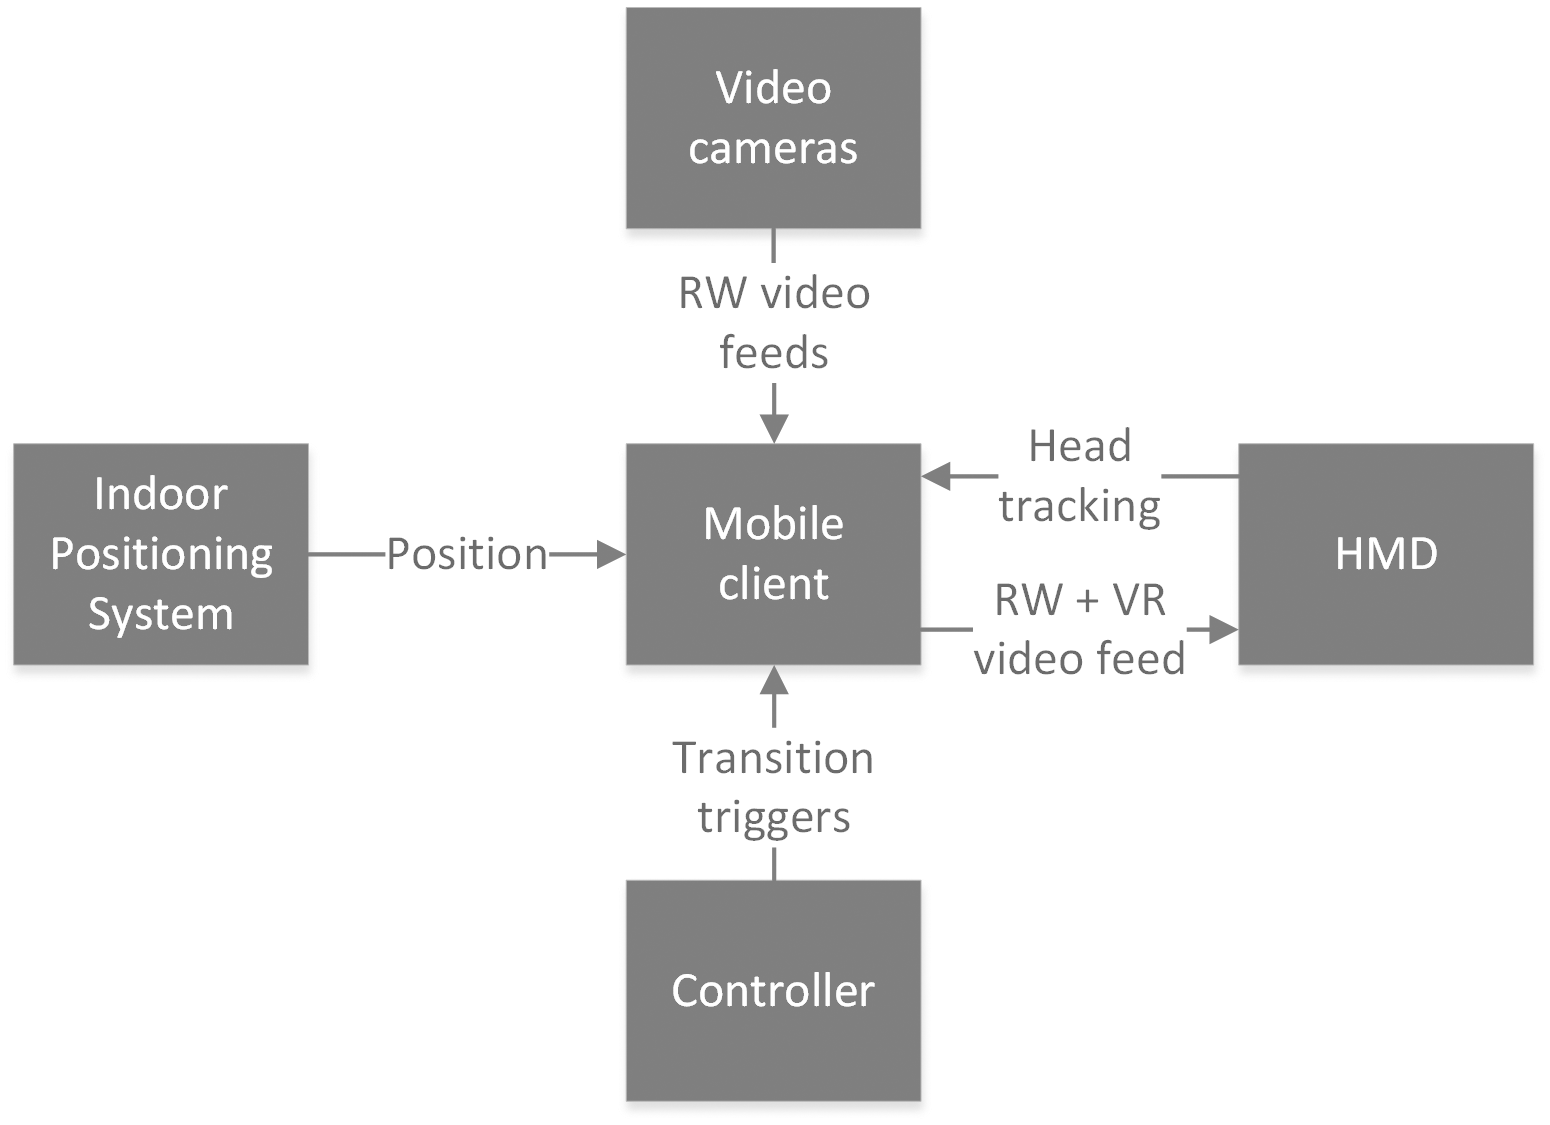
\includegraphics[width=.5\linewidth]{system-architecture.png}
		\caption{Overview of the Mirrorshades platform.}
		\label{systemarchitecture}
	\end{center}
\end{figure}

%=========================================================================================================

\section{Indoor Positioning}

PSMove - talk about how even in relatively dimly lit conditions (screencap video) it cannot track, so no chance in real world virtual heritage (or otherwise) conditions
	%https://www.youtube.com/watch?v=n_jGShUAqJg
	
\begin{figure}[h]
	\begin{center}
		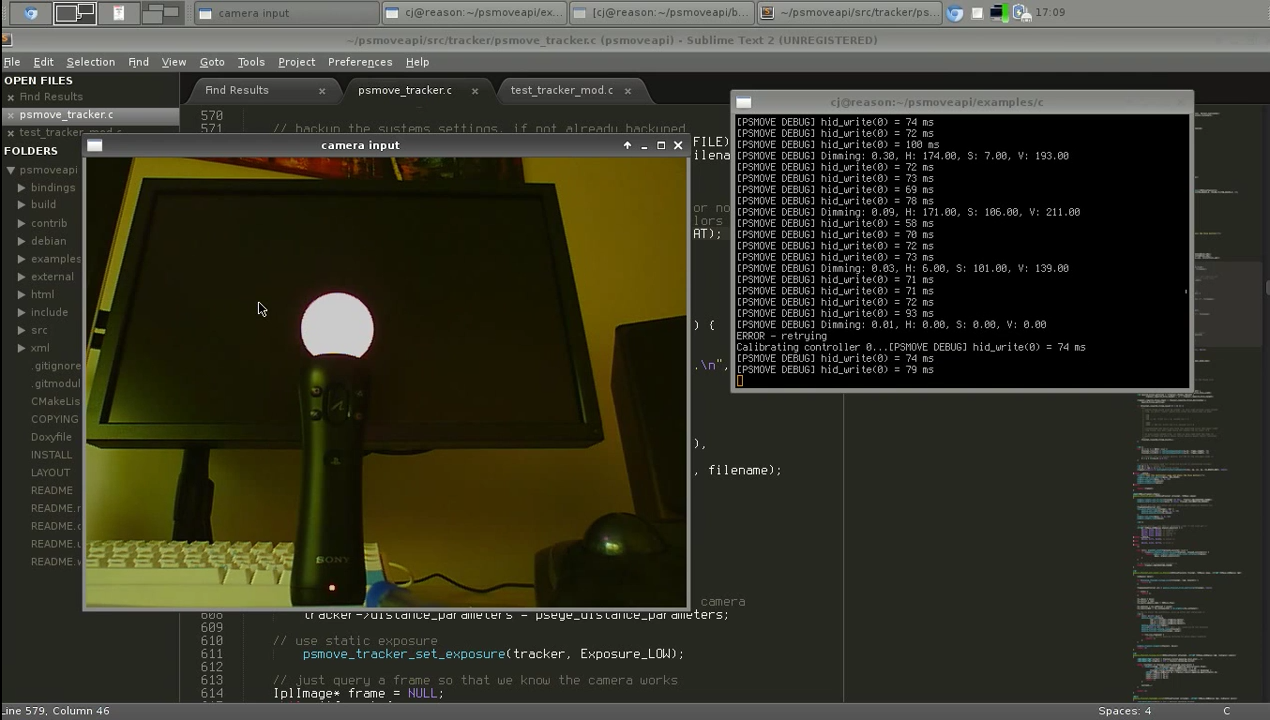
\includegraphics[width=.8\linewidth]{psmove-screenshot.png}
		\caption{psmove-screenshot.png}
		\label{psmove-screenshot.png}
	\end{center}
\end{figure}


Arduino ultrasonics

Habilitation thesis on indoor positioning systems\cite{Mautz2012}

Email from cricket guy

Indoor Atlas

%=========================================================================================================

\section{Modifying the Oculus Rift for Stereoscopic See Through Video}

\textbf{***Mention first Mirrorshades test with single webcam providing small floating window in corner of virtual view (video is on youtube/Mirrorshades repo).}

\newcommand{\floatingwebcamFootnote}{\footnote{\url{https://www.youtube.com/watch?v=tS0FGZxQzCU}}}

\begin{figure}[h]
	\begin{center}
		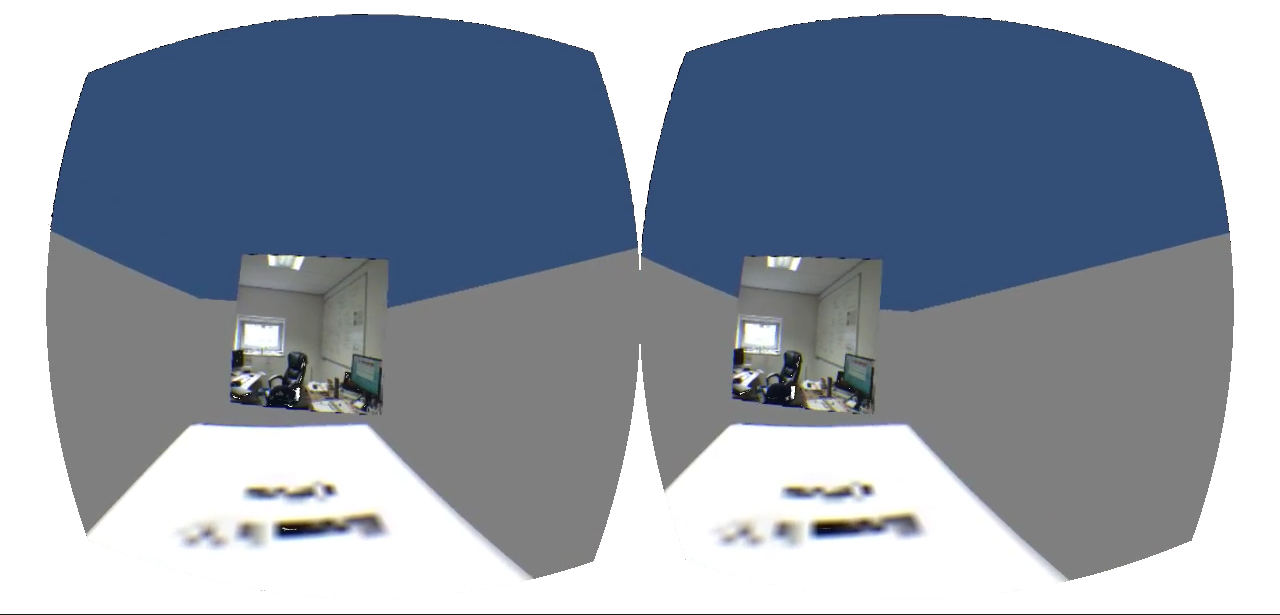
\includegraphics[width=0.7\textwidth]{floating_webcam_window.png}
		\caption{Early floating window Rift/webcam prototype.}
		\label{floating_webcam_window.png}
	\end{center}
\end{figure}

\textbf{**Show lens comparison picture from blog \& a (new?) screenshot showing FoV of the camera feeds compared to that of Rift \& explain why the discrepancy doesn't matter, especially when the Rift is fully extended.}

\begin{figure}[!htb]
    \centering
    \begin{minipage}{.32\textwidth}
        \centering
        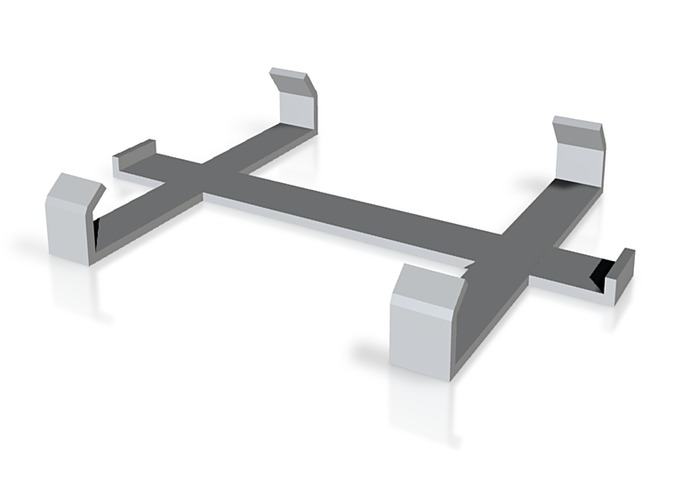
\includegraphics[width=\textwidth]{rift-clips-cameras/clips.jpg}
        \caption{bar}
        \label{bar}
    \end{minipage}%
    \hspace{.01\textwidth}
    \begin{minipage}{0.32\textwidth}
        \centering
        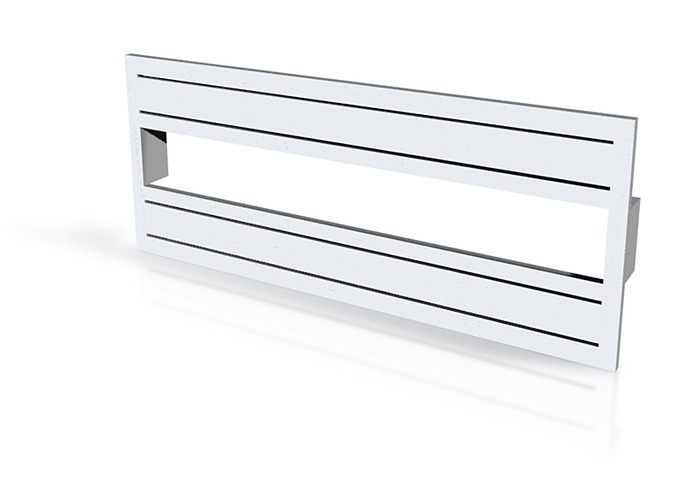
\includegraphics[width=\textwidth]{rift-clips-cameras/clips-hori-plate.jpg}
        \caption{foo}
        \label{foo}
    \end{minipage}%
    \hspace{.01\textwidth}
    \begin{minipage}{0.32\textwidth}
        \centering
        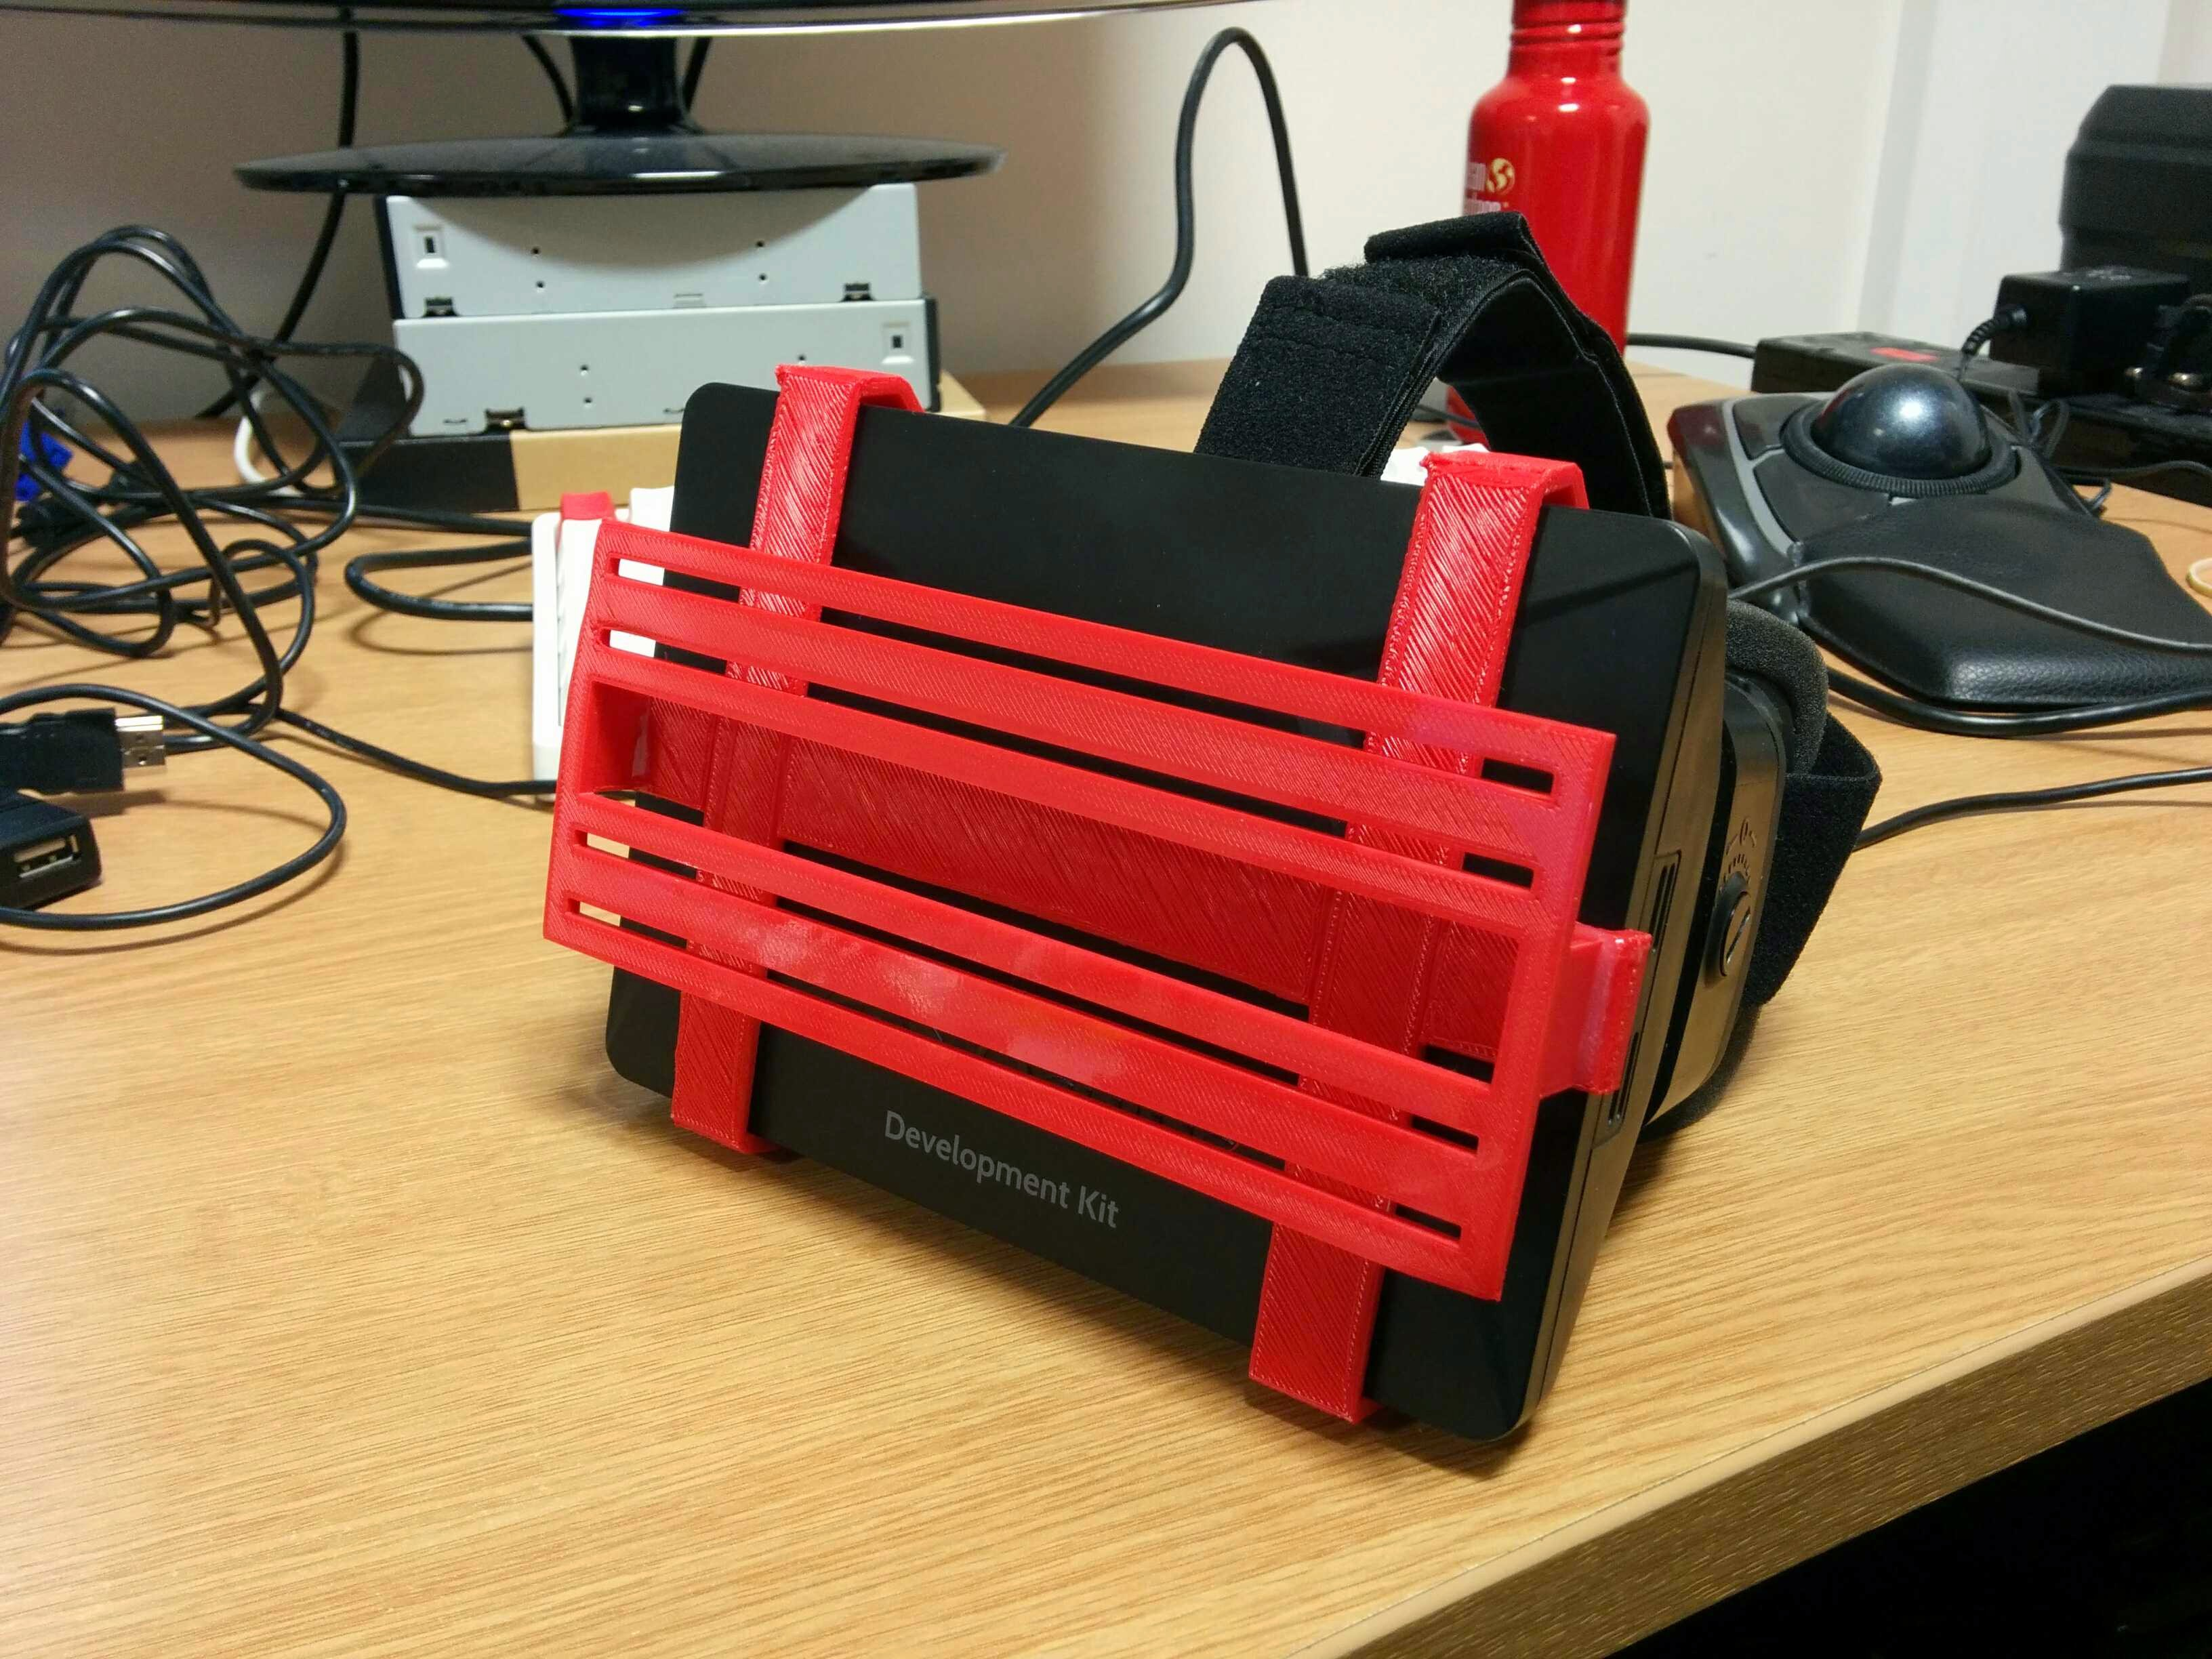
\includegraphics[width=\textwidth]{rift-clips-cameras/hori-1.jpg}
        \caption{baz}
        \label{baz}
    \end{minipage}
\end{figure}

\TwoFig{rift-clips-cameras/hori-2.jpg}{hori-2.jpg}{hori-2.jpg}
       {rift-clips-cameras/hori-3.jpg}{hori-3.jpg}{hori-3.jpg}

\TwoFig{rift-clips-cameras/lens-comparison-on-ps3eye-pcb.jpg}{lens-comparison-on-ps3eye-pcb.jpg}{lens-comparison-on-ps3eye-pcb.jpg}
       {rift-clips-cameras/lens-comparison.jpg}{lens-comparison.jpg}{lens-comparison.jpg}

\TwoFig{rift-clips-cameras/clips-vert.jpg}{clips-vert.jpg}{clips-vert.jpg}
       {rift-clips-cameras/vert-6.jpg}{vert-6.jpg}{vert-6.jpg}

\TwoFig{rift-clips-cameras/vert-1.jpg}{vert-1.jpg}{vert-1.jpg}
       {rift-clips-cameras/vert-4.jpg}{vert-4.jpg}{vert-4.jpg}

\TwoFig{rift-clips-cameras/thermoplastic.jpg}{thermoplastic.jpg}{thermoplastic.jpg}
       {rift-clips-cameras/vert-7.jpg}{vert-7.jpg}{vert-7.jpg}

\TwoFig{rift-clips-cameras/middle.jpg}{middle.jpg}{middle.jpg}
       {rift-clips-cameras/right.jpg}{right.jpg}{right.jpg}

\TwoFig{latency/vid1.jpg}{vid1.jpg}{vid1.jpg}
       {latency/vid2.jpg}{vid2.jpg}{vid2.jpg}

\TwoFig{latency/vid3.jpg}{vid3.jpg}{vid3.jpg}
       {latency/vid4.jpg}{vid4.jpg}{vid4.jpg}

\begin{figure}[h]
    \begin{center}
    \begin{minipage}{.32\textwidth}
        \begin{center}
        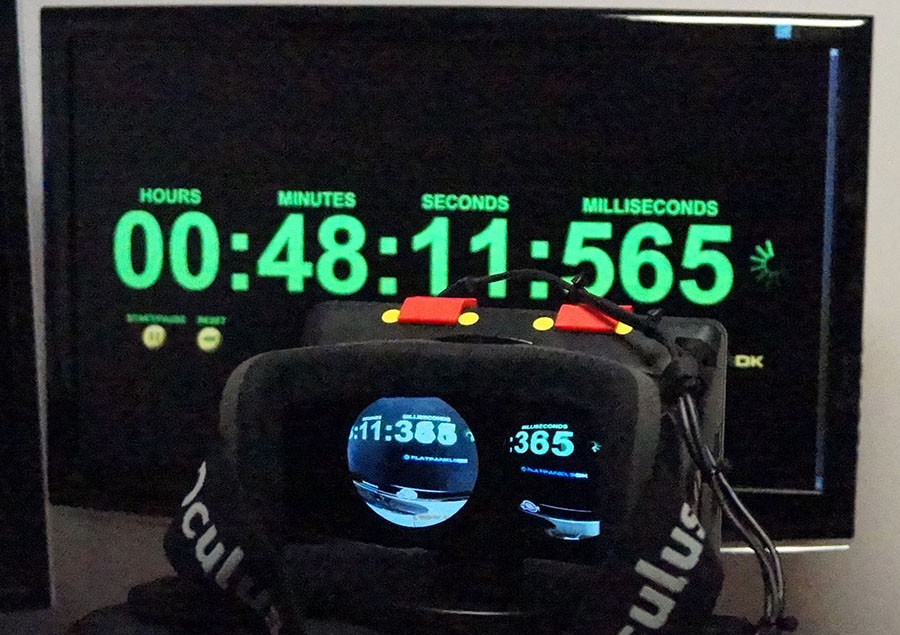
\includegraphics[width=\textwidth]{latency/still1.jpg}
        \caption{still1.jpg}
        \label{still1.jpg}
        \end{center}
    \end{minipage}%
    \hspace{.01\textwidth}
    \begin{minipage}{.32\textwidth}
		\begin{center}
        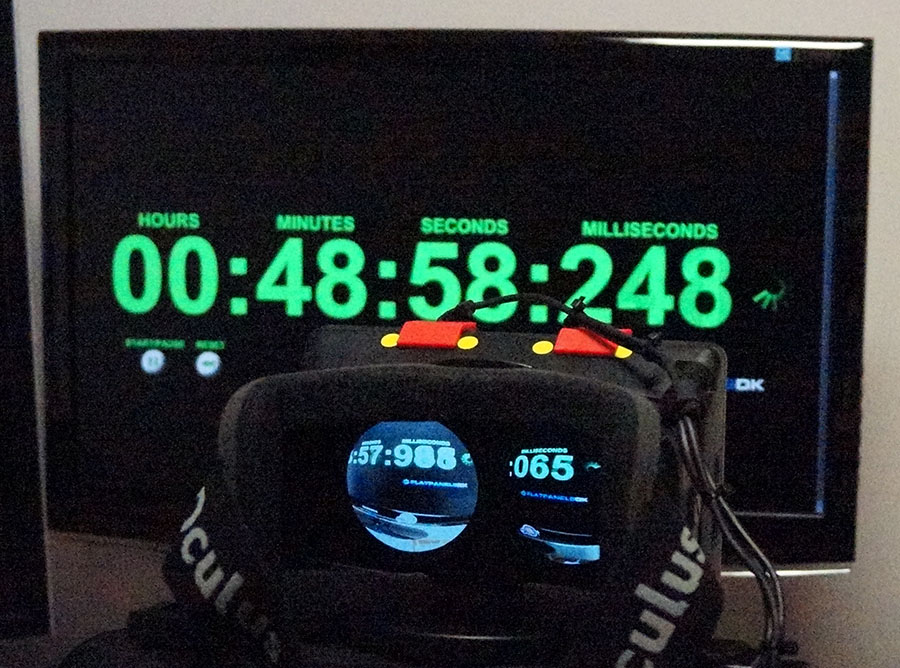
\includegraphics[width=\textwidth]{latency/still2.jpg}
        \caption{still2.jpg}
        \label{still2.jpg}
        \end{center}
    \end{minipage}%
    \hspace{.01\textwidth}
    \begin{minipage}{.32\textwidth}
        \begin{center}
        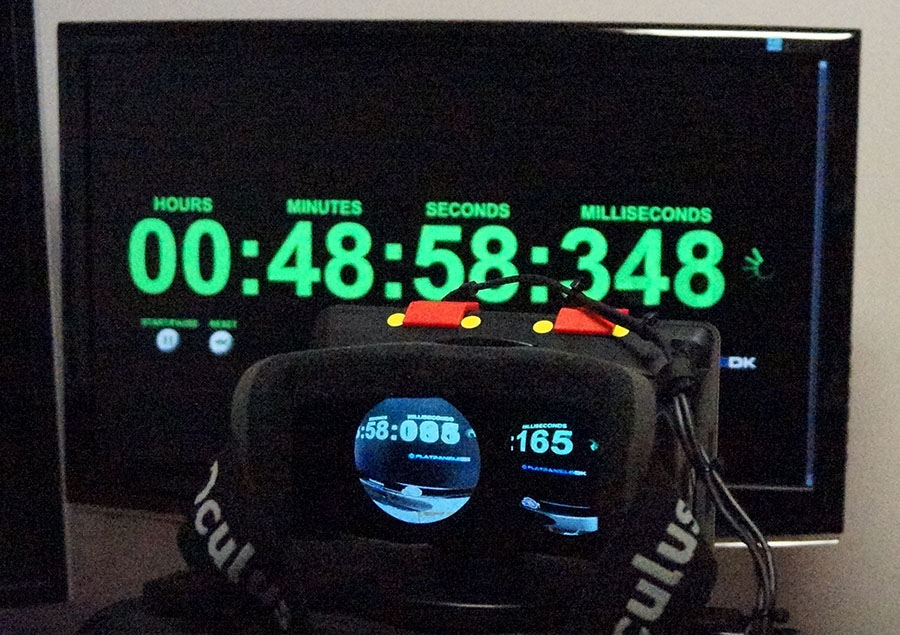
\includegraphics[width=\textwidth]{latency/still3.jpg}
        \caption{still3.jpg}
        \label{still3.jpg}
        \end{center}
    \end{minipage}
    \end{center}
\end{figure}

%=========================================================================================================

\section{Platform}

Talk about trying Oculus on Android (ODROID) \& how now Samsung Gear VR would be ideal, but yolo laptop in a bag. Photo of ODROID/screencap of (\& link to) video showing Rift working (at least tracking) with ODROID?

%=========================================================================================================

\subsection{Implementation}
Figure \ref{experimentalimplementation} presents an overview of the implementation of the Mirrorshades platform design for use in the chapel investigations.

\begin{figure}[h]
	\thispagestyle{empty}
	\begin{center}
		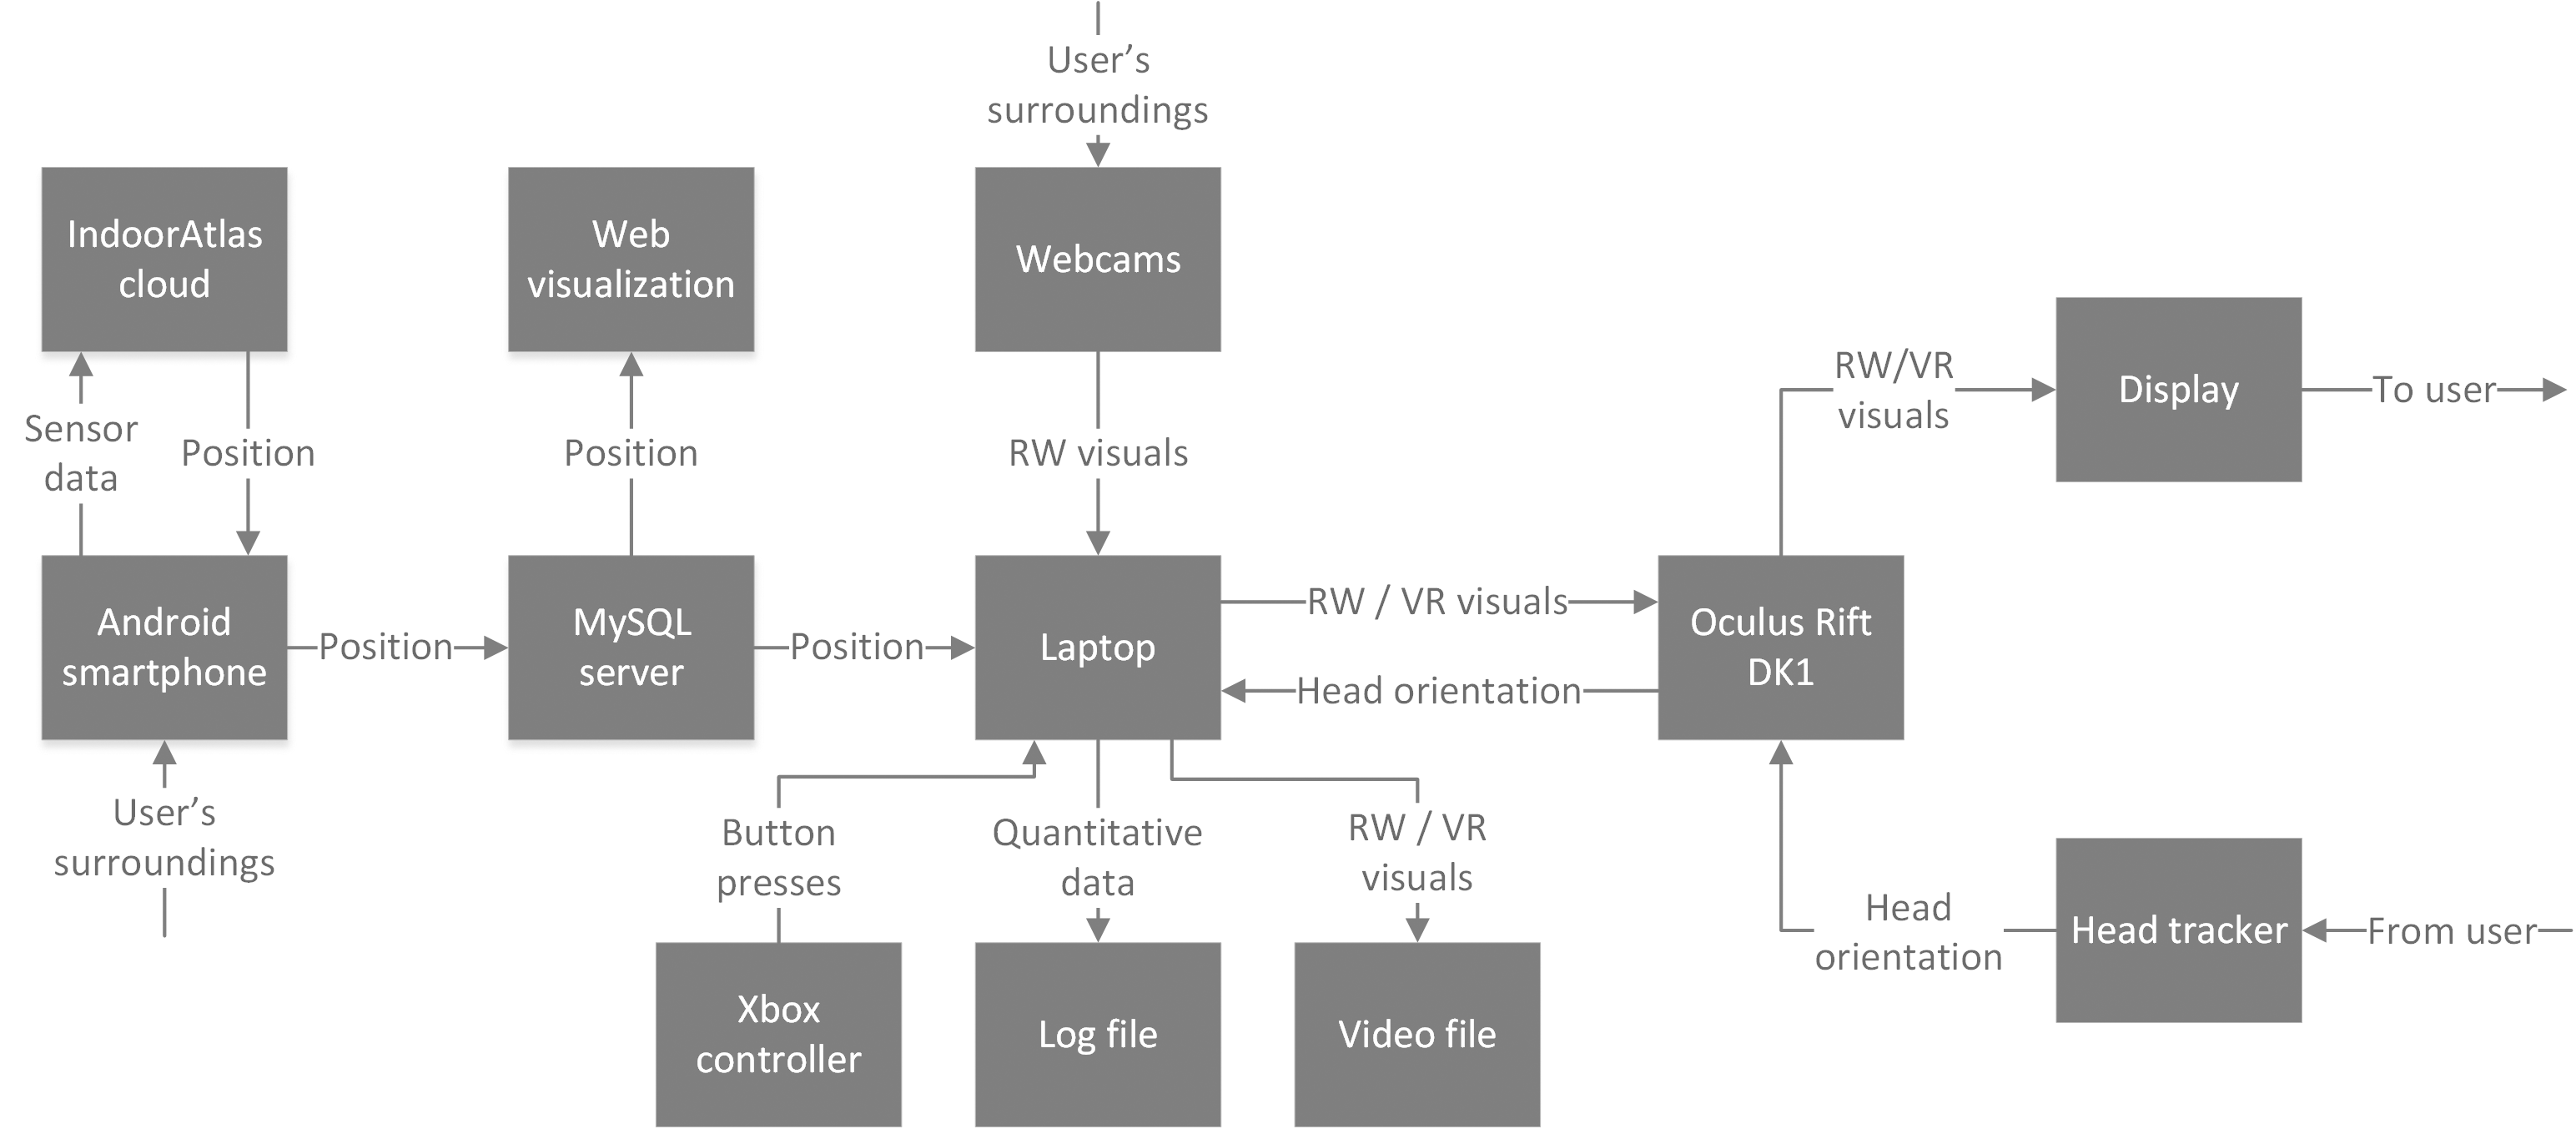
\includegraphics[width=.925\linewidth]{experimental-implementation.png}
		\caption{Implementation of Mirrorshades platform.}
		\label{experimentalimplementation}
	\end{center}
\end{figure}

%=========================================================================================================

\subsection{Hardware Components}
The hardware of the implementation comprises;

\begin{itemize}
	\item an Oculus Rift DK1 HMD, including a 9-axis (3dof rotational) head tracker sampling at 1000Hz \& mounted with a stereo camera solution comprising 2x Logitech C310 webcams modified with M12 lens mounts \& 2.1mm lenses to provide approximately 87 degrees horizontal FOV of the RW environment (see figure \ref{rift});
	\item a USB battery pack, to power the HMD;
	\item a small laptop computer, with an Intel i7-3632QM processor, Nvidia GT 650M graphics card \& 16GiB system memory;
	\item an Android smartphone, running Android 4.4.4;
	\item an Xbox 360 wireless controller, with USB receiver.
\end{itemize}

%\begin{figure}[h]
%	\begin{center}
%		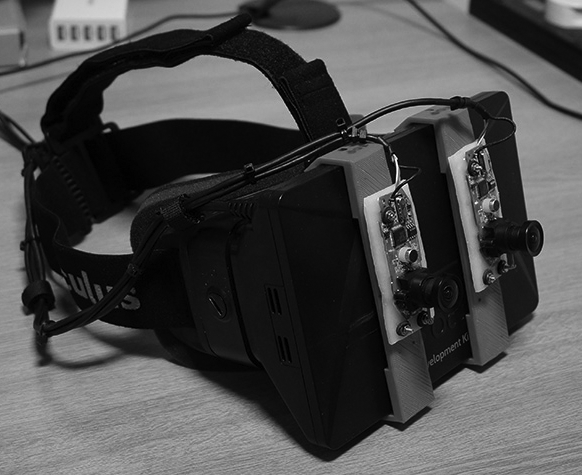
\includegraphics[width=0.6\textwidth]{rift.png}
%		\caption{HMD with stereo camera solution.}
%		\label{rift}
%	\end{center}
%\end{figure}

%=========================================================================================================

\subsection{Software Components}
The software of the implementation comprises;

\begin{itemize}
	\item an Android application that runs on the smartphone, determines the location of the phone within the building that it is in using the IndoorAtlas IPS~\cite{IndoorAtlasLtd.2012} (figure \ref{sallies_layout} shows the paths within the chapel upon which the IPS has been configured) \& submits these location data via PHP to a database server;
	\item a MySQL database server that stores location data for the phone \& allows these data to be accessed both by the Unity application running upon the laptop \& by a web visualisation;
	\item a Unity application that runs on the laptop.
\end{itemize}

%=========================================================================================================

\subsection{Integration of Components}
The Unity application hosts the VR representation of the chapel \& takes in feeds from both webcams, the HMD head tracker \& the Xbox controller. It also polls the database server for the most recent position data. All of these inputs are combined together to form the visual output for the HMD to display to the user.

As the user moves their head, the visuals that are presented to them upon the HMD's display change accordingly; the RW visuals change due to the webcams being physically fixed to the HMD \& the VR visuals change due to data from the head tracker being used to change the orientation of the in game `cameras' accordingly.

As the user changes their position by walking, the visuals that are presented to them upon the HMD's display also change accordingly; again the RW visuals change due to the webcams' position upon the HMD whilst the VR visuals change due to the user's position, as reported by the smartphone \& the IndoorAtlas solution, being used to move the position of the in game cameras to the equivalent position within the VR representation.

As the user presses buttons or pulls triggers upon the Xbox controller, the visuals that are presented to them upon the HMD's display transition between RW \& VR in different styles depending upon which button/trigger was activated.

%=========================================================================================================

\subsection{Transition Methods}
Attending to visual stimuli from the RW environment via the webcams is required for the user to safely move around. Delay in the IPS reporting their position \& inaccuracies in these position data (see figure \ref{jack-cole-splodges} for a set of example position data) mean that moving around while attending only to visual stimuli from the VR environment would not be safe for the user, even with unchanging RW obstacles with perfectly accurate representations in the VR environment. Furthermore it is actually likely that RW obstacles will not have equivalent VR representations, such as in a scenario where XR is used to compare \& contrast changes to a building's interior over extended periods of time (such as with the chapel investigations).

\begin{figure}[h]
	\begin{center}
		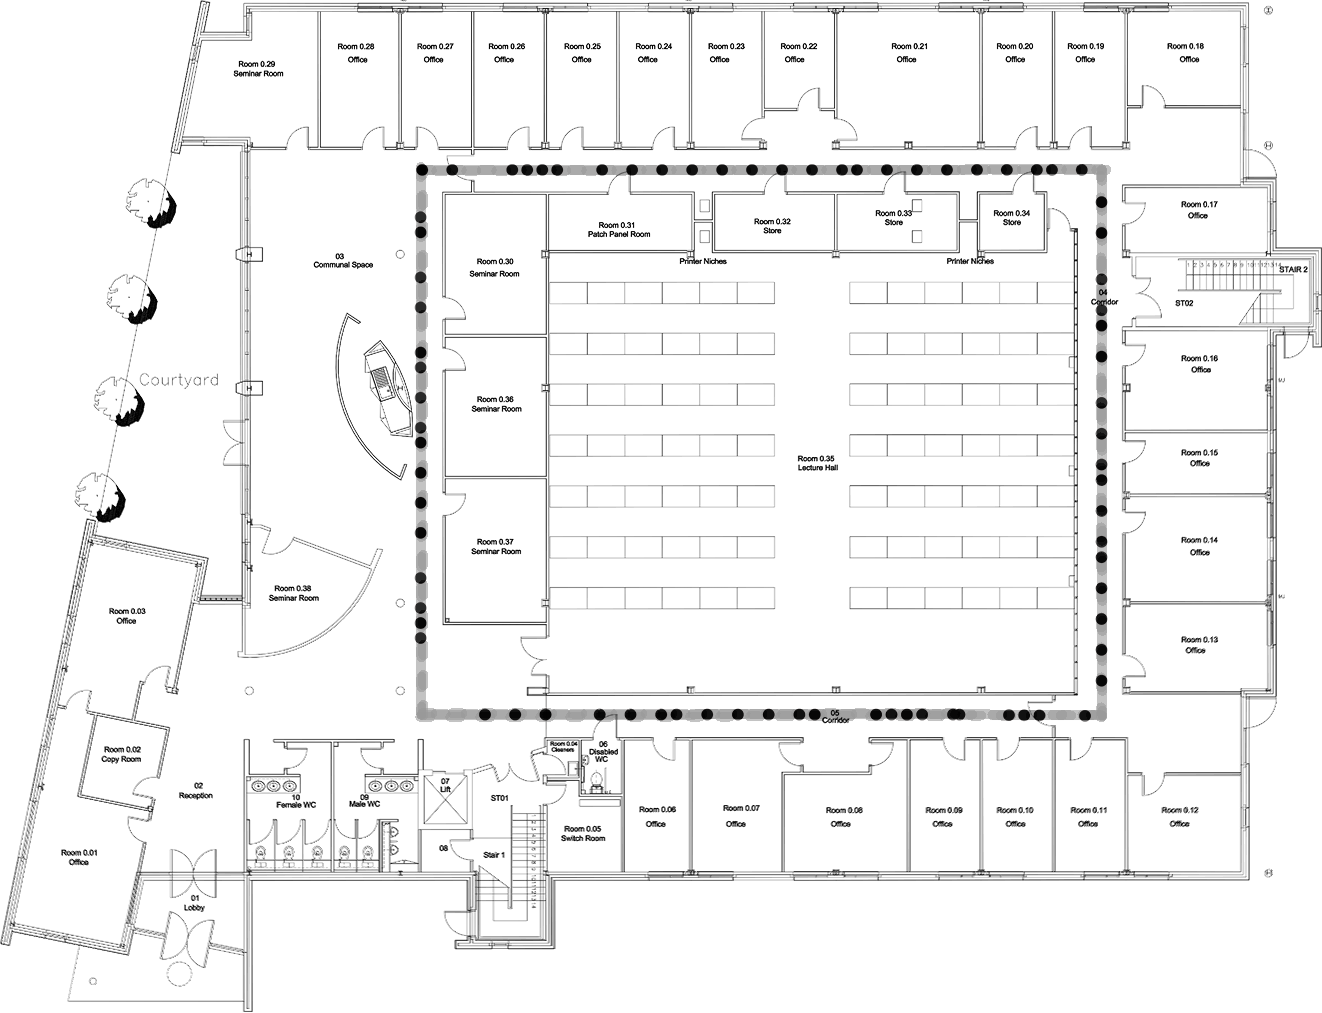
\includegraphics[width=0.7\textwidth]{jack-cole-splodges-black.png}
		\caption{Positions (black circles) reported whilst walking a slow lap ($<1$ms$^{-1}$, following gray path) of a departmental building. The building is approximately 40m wide by 30m tall.}
		\label{jack-cole-splodges}
	\end{center}
\end{figure}

Thus the HMD displays the feeds from the webcams as default \& the user must trigger transitions to view the VR environment by pressing a button or pulling a trigger on the controller. Releasing the button/trigger causes the webcam feeds to be displayed again.

%=========================================================================================================

\subsubsection{Hard switch}
\label{sub-hardswitch}
The user presses \& holds the \texttt{[A]} button on the controller to switch the visual stimuli displayed by the HMD from RW to VR. When the \texttt{[A]} button is released, the visual stimuli displayed by the HMD switch back from VR to RW. This is a `hard' or `immediate' switch with no fading or transition effect. Figure \ref{scenario1} illustrates this scenario.

\begin{figure}[h]
	\begin{center}
		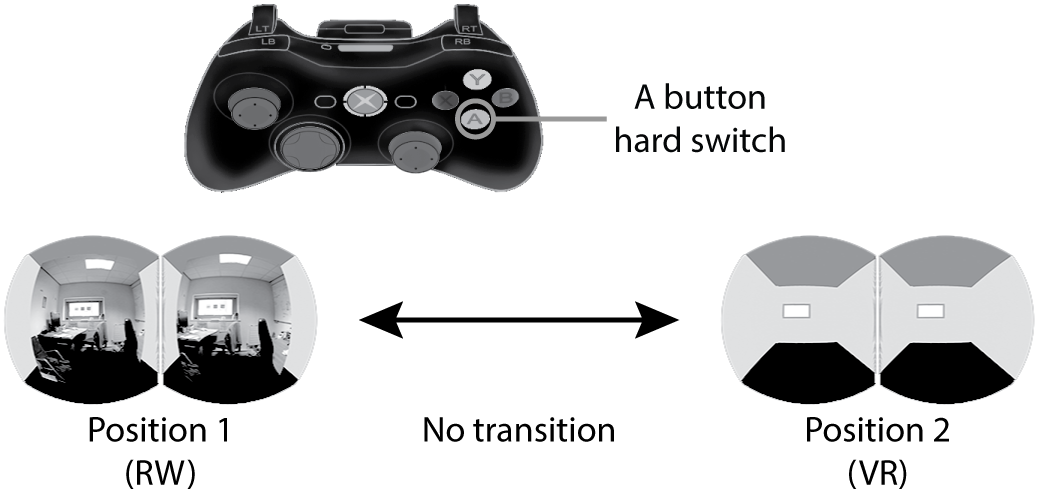
\includegraphics[width=0.7\textwidth]{switching-hard-with-controller.png}
		\caption{Hard switch.}
		\label{scenario1}
	\end{center}
\end{figure}

%=========================================================================================================

\subsubsection{Switch with linear interpolation}
The user presses \& holds the \texttt{[B]} button on the controller to switch the visual stimuli displayed by the HMD from RW to VR. When the \texttt{[B]} button is released, the visual stimuli displayed by the HMD switch back from VR to RW. This switch fades between RW \& VR  visual stimuli using linear interpolation on the opacity of the game objects that the webcam feeds are rendered upon. Figure \ref{scenario12} illustrates this scenario.

\begin{figure}[h]
	\begin{center}
		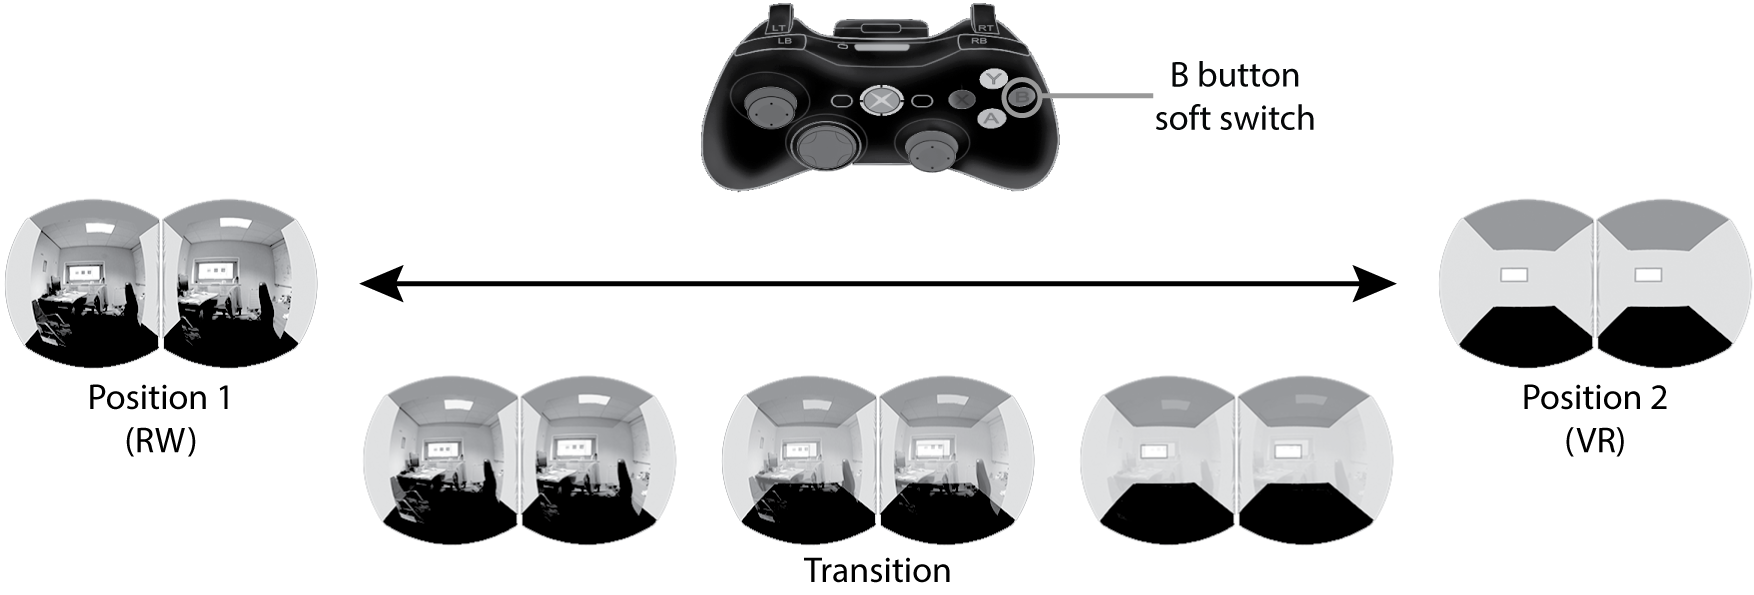
\includegraphics[width=\textwidth]{switching-soft-with-controller.png}
		\caption{Switch with linear interpolation.}
		\label{scenario12}
	\end{center}
\end{figure}

%=========================================================================================================

\subsubsection{Analogue selectable opacity}
The user pulls the right analogue trigger (\texttt{[RT]}) on the controller, where the position of the trigger maps directly to the opacity of the game objects that the webcam feeds are rendered upon. The user can choose to stop at any intermediary position that suits their needs, keeping the level of opacity of the webcam feeds at that position, as well as controlling the rate at which the visual stimuli from the RW environment fade (by changing how quickly they change their depression of the trigger). Pulling the trigger all the way in displays only visual stimuli from the VR environment, while releasing it completely displays only visual stimuli from the RW environment. The number of intermediary positions is limited only by the resolution of the trigger \& the encoding of the value.

This method allows the user to superimpose VR visual stimuli upon RW visual stimuli. This is similar, but not identical, to AR, as instead of displaying a small number of virtual objects upon the user's view of their RW environment, a complete VR environment is superimposed upon the user's view of their RW environment. Figure \ref{scenario2} illustrates this scenario.

\begin{figure}[h]
	\begin{center}
		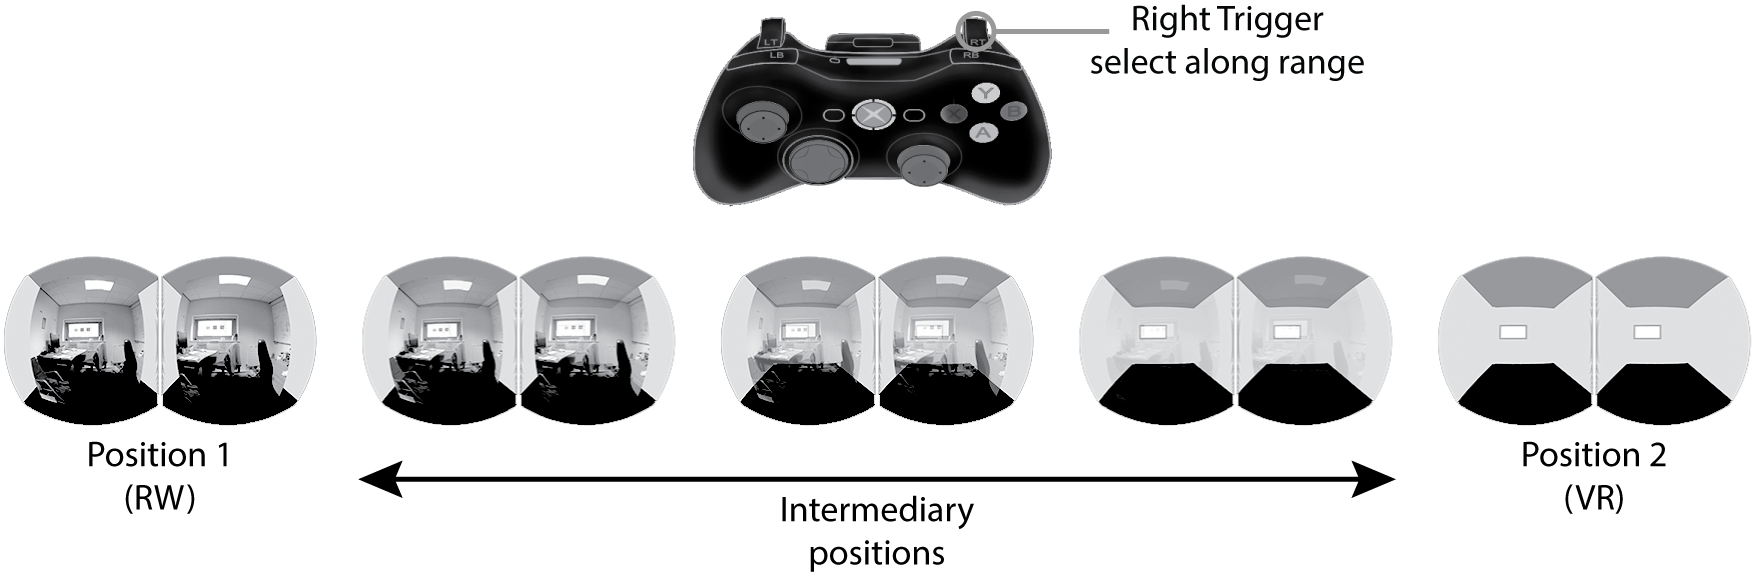
\includegraphics[width=.9\textwidth]{switching-analogue-with-controller.png}
		\caption{Analogue selectable opacity.}
		\label{scenario2}
	\end{center}
\end{figure}

%=========================================================================================================

\subsubsection{Periodic hard switches}
\label{subsub-periodic}
Independent or in addition to any of the previous scenarios, the visual stimuli displayed by the HMD switch from RW to VR at a set interval \& for a set amount of time. For example, every 3 seconds the stimuli switch from RW to VR for 0.2 of a second before switching back from VR to RW. Any user triggered transitions cause the interval timer to be reset, such that an `automated' switch will never occur after less time from a user triggered switch than the set interval. Automated transitions are disabled whilst \texttt{[RT]} is at all depressed. Figure \ref{scenariotimed} illustrates this scenario, where \texttt{i} represents the interval between switches \& \texttt{d} represents the duration of the switch from RW to VR.

\begin{figure}[h]
	\begin{center}
		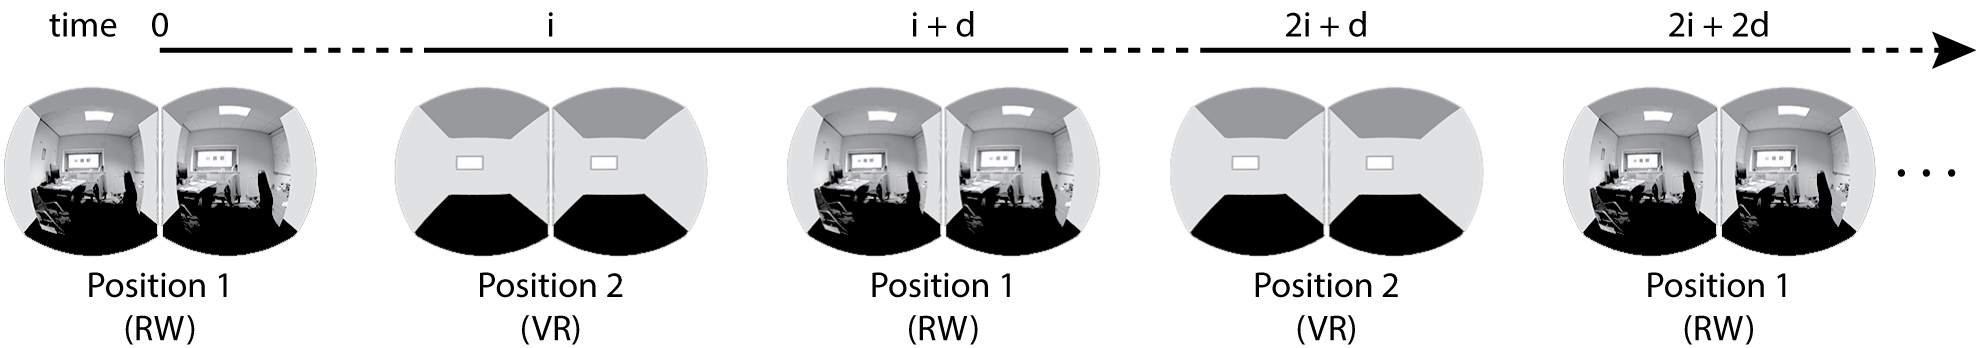
\includegraphics[width=\textwidth]{timed-switch.png}
		\caption{Periodic hard switches.}
		\label{scenariotimed}
	\end{center}
\end{figure}

%=========================================================================================================

\subsubsection{Reduced maximum opacity}
\label{subsub-baseopacity}
Independent or in addition to any of the previous scenarios, the maximum opacity of the game objects that the webcam feeds are rendered upon is reduced, such that the `default' position at which a transition has not been triggered (either by a button press, trigger movement or by a periodic switch) displays VR superimposed upon RW. Figure \ref{scenariobaseopacity} illustrates this scenario in combination with a hard switch (from section \ref{sub-hardswitch}) in which the user triggers hard switches between the default position of a superimposition of VR upon RW \& a position where only VR stimuli are present.

\begin{figure}[h]
	\begin{center}
		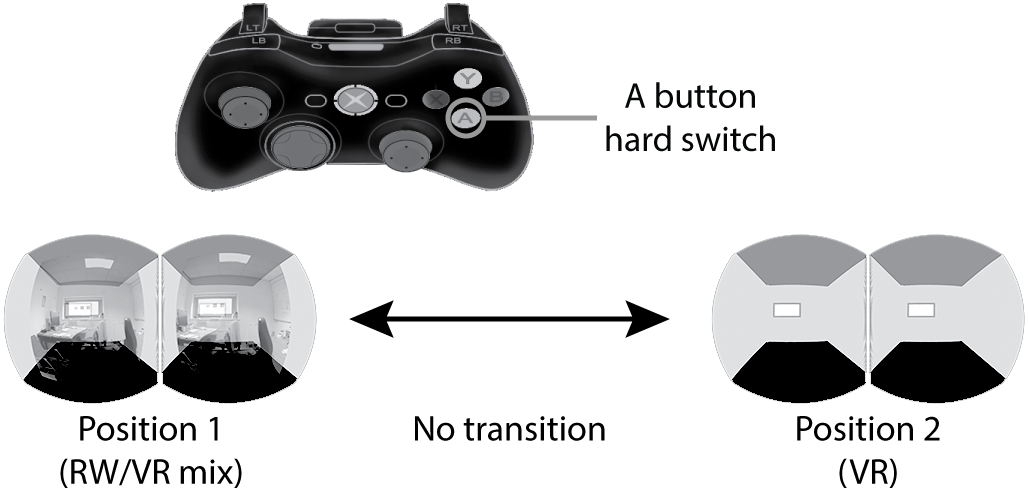
\includegraphics[width=0.7\textwidth]{base-opacity-hard-switch.png}
		\caption{Hard switch from reduced maximum opacity.}
		\label{scenariobaseopacity}
	\end{center}
\end{figure}

%=========================================================================================================





















%=========================================================================================================

%\textit{Two different buildings have been prepared for use with the Mirrorshades platform, with VR environments constructed \& the IndoorAtlas IPS deployed. The first is a modern building accompanied by a VR environment that closely depicts it in the present day. The second is a historic building accompanied by a VR environment that differs markedly from the present day, by depicting its state a point hundreds of years in the past.}

%\textit{In the first, participants will be given a simple task to complete which will encourage them to engage with the VR environment even though it presents a similar view to their RW environment. In the second scenario, participants will be prompted to engage in more free form exploration of their environments, comparing \& contrasting the markedly different VR environment with what they see around them in their RW environment.}

%\subsection{Jack Cole Building}
%The School of Computer Science Jack Cole building at St Andrews is a modern building, built in 2004. The VR environment accompanying the building is a fairly close representation of the building as it stands today. Figure \ref{jc_layout} shows the layout of the building \& the path that IndoorAtlas has been prepared for.

%There are four coloured panels (red, green, blue \& yellow) situated within the VR building upon walls, floor \& ceiling. Participants will be asked to remember in what order these panels are seen as they walk a lap of the building. This task is designed to encourage participants to switch between RW \& VR visual stimuli, even though the VR visual stimuli are very similar to those of the RW environment. This scenario is also intended to encourage participants to keep moving, rather than stopping at \& starting.

%\begin{figure}[h]
%	\begin{center}
%		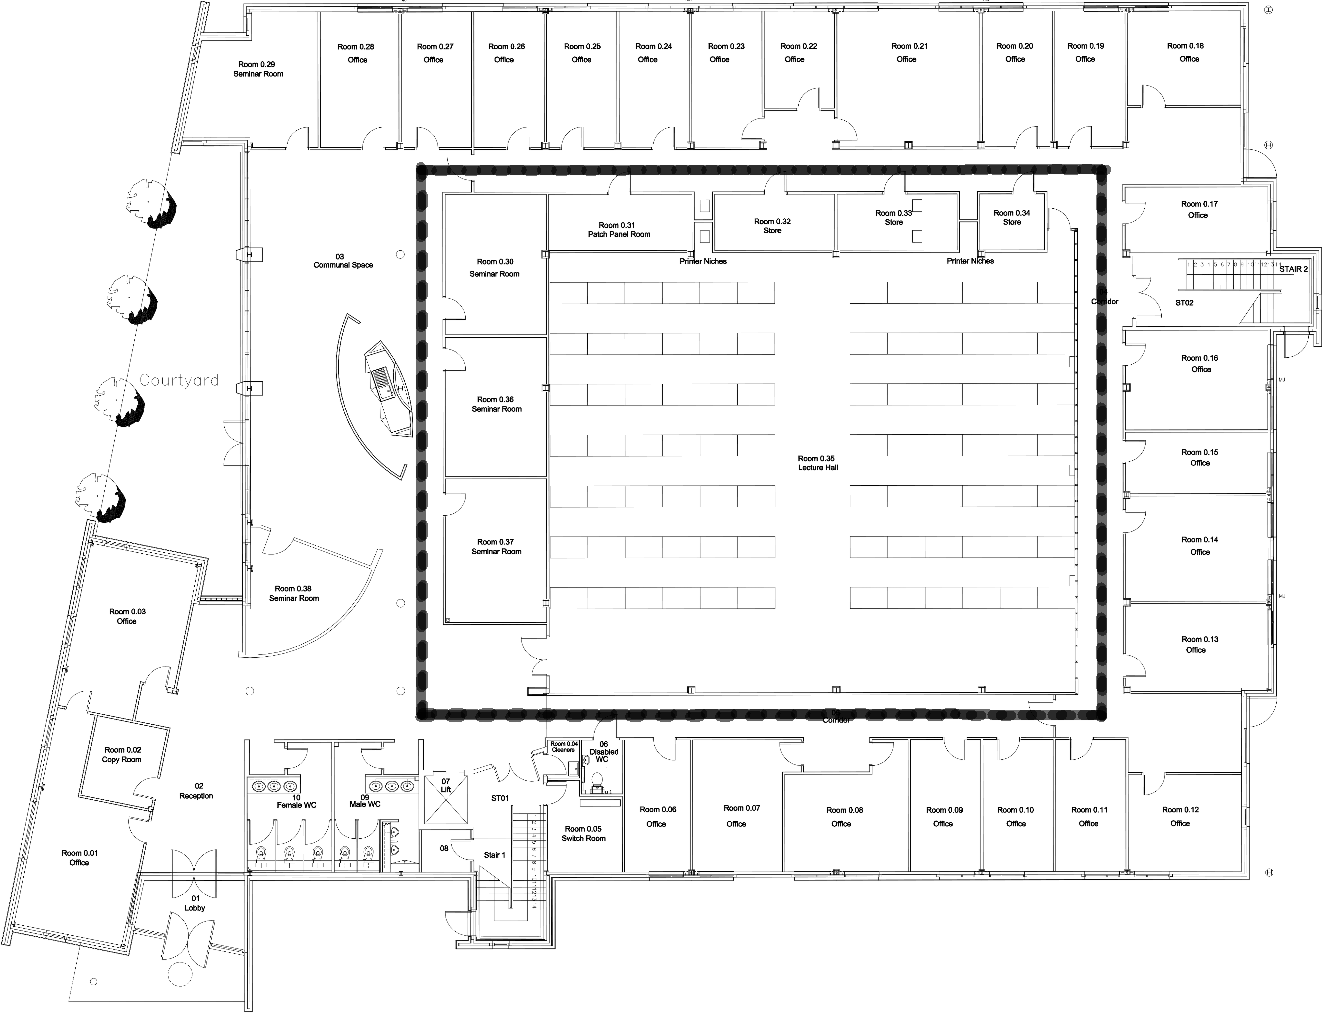
\includegraphics[width=0.7\textwidth]{JC_layout.png}
%		\caption{Floor plan of Jack Cole building, with IPS route.}
%		\label{jc_layout}
%	\end{center}
%\end{figure}

%=========================================================================================================